\documentclass{beamer}
\usepackage[T1]{fontenc}
\usepackage{textcomp}
\usepackage[utf8]{inputenc}
\usepackage[danish]{babel}
\usepackage[garamond]{mathdesign}
\usepackage{url}
\usepackage{listings}
\usepackage{graphicx}
\usepackage{soul}

\renewcommand{\ttdefault}{pcr} % bedre typewriter font
\renewcommand{\rmdefault}{ugm} % garamond
\renewcommand{\sfdefault}{phv} % sans-serif font

\title{Hjemmesideanalyse}
\subtitle{Førsteårsprojekt}

\author{Martin Dybdal \and Troels Henriksen \and Jesper Reenberg}

\institute{\textrm{Datalogisk Institut, Københavns Universitet}}
\date{\today}

\mode<presentation>
{
  \usetheme{Frankfurt}
  %\usetheme{Warsaw} 
  \definecolor{uofsgreen}{rgb}{.125,.5,.25}
  \definecolor{natvidgreen}{rgb}{.196,.364,.239}
  \definecolor{kugrey}{rgb}{.4,.4,.4}
  \usecolortheme[named=uofsgreen]{structure}
  \usefonttheme[onlylarge]{structuresmallcapsserif}
  \usefonttheme[onlysmall]{structurebold}
}

\logo{
\includegraphics[height=1.5cm]{diku.jpg}}

\usenavigationsymbolstemplate{} % fjern navigation

\lstloadlanguages{HTML}
\lstset{language     = ML,
        extendedchars= true,
        breaklines   = false,
        tabsize      = 2,
        showstringspaces = false,
        basicstyle   = \small\ttfamily,
        commentstyle = \em,
        inputencoding= utf8
      }

\setcounter{tocdepth}{1}

\begin{document}

\frame{\titlepage}


\section{Introduktion}
\subsection{Agenda}
\begin{frame}
  \frametitle{Agenda}
  \tableofcontents
\end{frame}

\subsection{Problemstilling}
\begin{frame}
  \frametitle{Problemstilling}

  \begin{itemize}
  \item<1-> Hjemmesider forfattet uden omtanke for læsbarhed
  \item<2-> Hjemmesider forfattet med primitive værktøjer
    \begin{itemize}
      \item<2-> Ingen stavekontrol
      \item<2-> Ingen grammatikkontrol
    \end{itemize}
  \item<3-> Store websteder kan være uoverskuelige at læsbarheds-vurdere manuelt
  \end{itemize}
\end{frame}

\section{Analyse} % anden overskrift evt. ?
\subsection{Målgruppe}
\begin{frame}
  \frametitle{Målgruppe}
  \begin{itemize}
  \item<1-> Webmastere
  \item<2-> Hjemmeside--skribenter
  \item<3-> \textbf{Mere generelt, brugbart for HTML-kyndige}
  \end{itemize}

\end{frame}

\subsection{Målgruppens behov}
\begin{frame}
  \frametitle{Målgruppens behov}
  \begin{itemize}
  \item<1-> Hele websteder skal analyseres
  \item<2-> Skal være let at finde læsbarhedsproblemer
  \item<3-> Store websteder, analyseresultater skal kunne deles
  \item<4-> Automatiseret programkørsel (via \texttt{cron} mfl.)
  \item<5-> Skal være muligt at finde problematiske undersider på store websteder
    \begin{itemize}
    \item<6-> Hver side skal tildeles en enkelt talværdi der angiver dens læsbarhed
    \end{itemize}    
  \end{itemize}
\end{frame}

\subsection{Præsentationsform}
\begin{frame}
  \frametitle{Præsentationsform}
  \begin{itemize}
    \item<1->HTML--dokumenter
      \begin{itemize}
      \item<1-> Kan deles.
      \item<2-> Intet behov for specifikt fremvisningsprogram.
      \item<3-> Webapplikation kan bygges ovenpå.
      \end{itemize}  

    \item<4->Kommandolinjeprogram
      \begin{itemize}
      \item<4-> Let at automatisere.
      \item<5-> \st{Let} overkommeligt at skrive grafisk interface.
      \end{itemize}  
    \end{itemize}
\end{frame}

\section{Design \& Implementering}
\subsection{Dataflow}
\begin{frame}
  \frametitle{Dataflow}
  \begin{figure}
    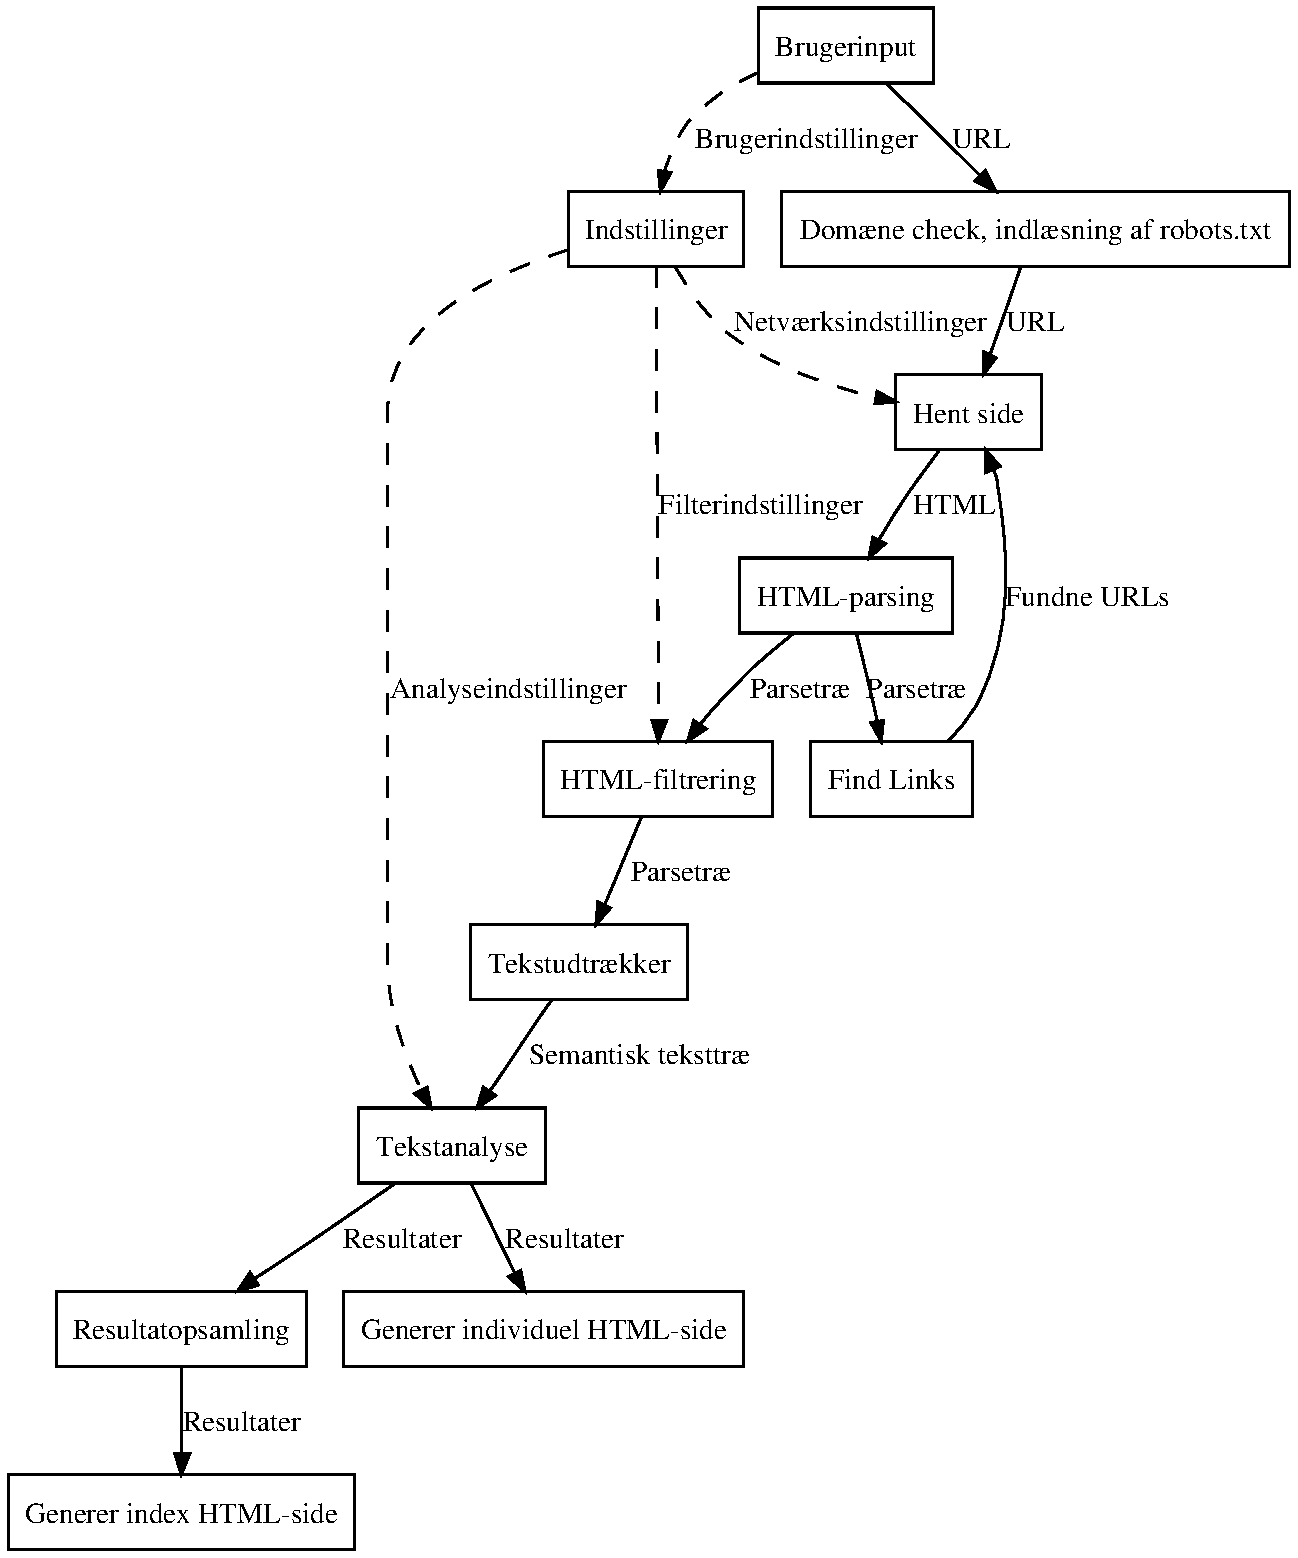
\includegraphics[width=0.55\textwidth]{endeligtdesignill.pdf}
  \end{figure}
\end{frame}

\subsection{HTML--Parsing}
\begin{frame}[fragile]
  \frametitle{HTML--Parsing}

  \begin{columns}[t]
    \column{.4\textwidth}
    \begin{figure}
\begin{lstlisting}[language=HTML, basicstyle=\tiny\ttfamily,
                   escapechar=\@]
<HTML>
  <HEAD>
    <TITLE>Sidetitel</TITLE>
  </HEAD>
  <!-- En kommentar -->
  <BODY>
    <P>
     Et afsnit med adskillige s@\ae@tninger.
     Dette er 'den anden s@\ae@tning'.
     </P>
    <BLOCKQUOTE lang="en">
     <A href="http://en.wikipedia.org/wiki/Hovercraft">
     My hovercraft</A> is full of eels!
    </BLOCKQUOTE>
  </BODY>
</HTML>
\end{lstlisting}

      \caption{HTML--dokument}
    \end{figure}

\pause

    \column{.6\textwidth}
    \begin{figure}
      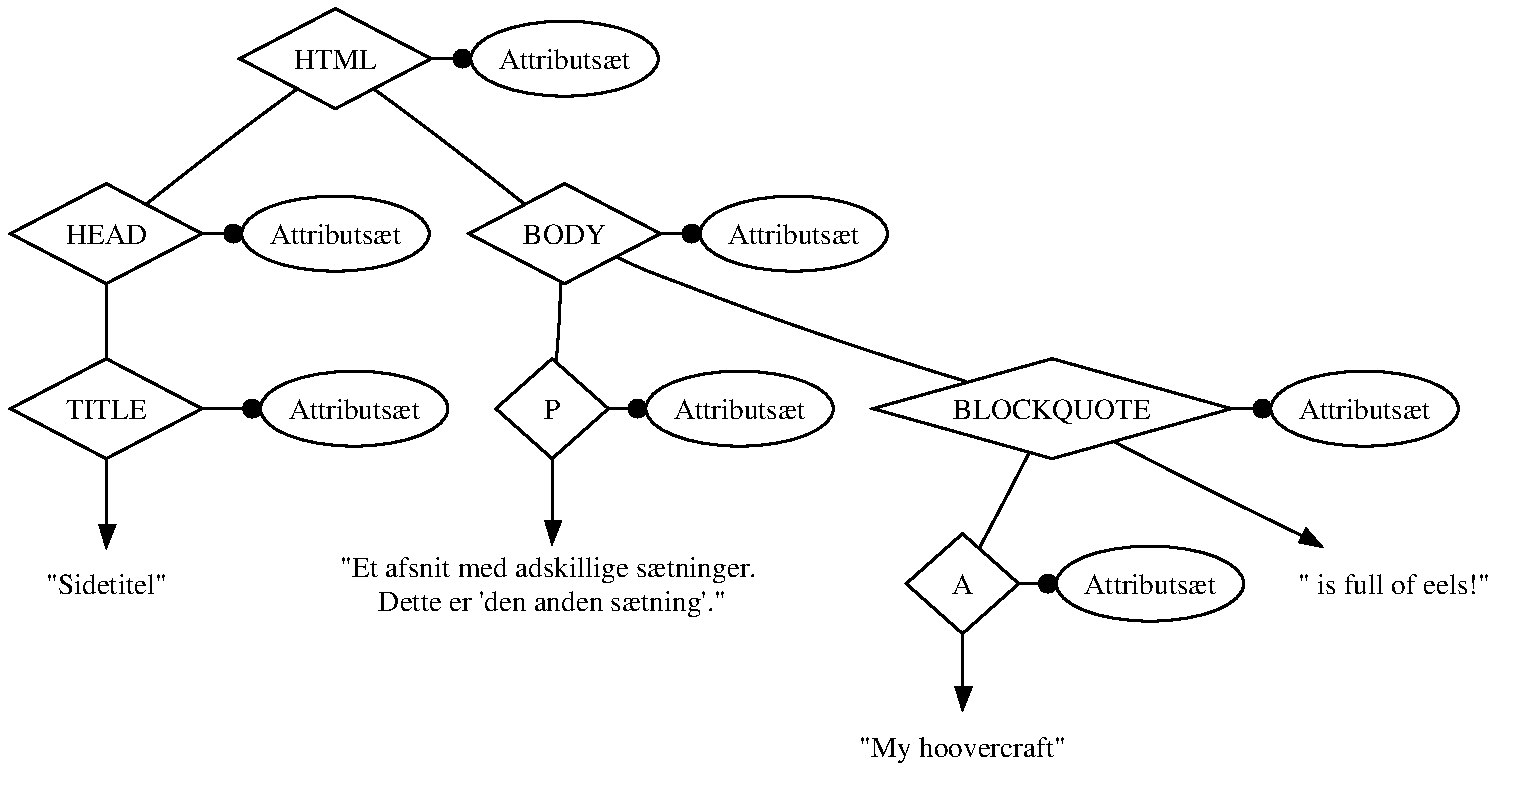
\includegraphics[width=\textwidth]{parsetree.pdf}
      \caption{Parsetræ}
    \end{figure}

    \begin{itemize}
    \item<1-> Beholder struktur
    \item<2-> Beholder data
    \end{itemize}
    
  \end{columns}

\end{frame}

\subsection{Tekstudtrækker}
\begin{frame}
  \frametitle{Udtræk af tekst}

  \begin{columns}[t]
    \column{.5\textwidth}
    \begin{figure}
      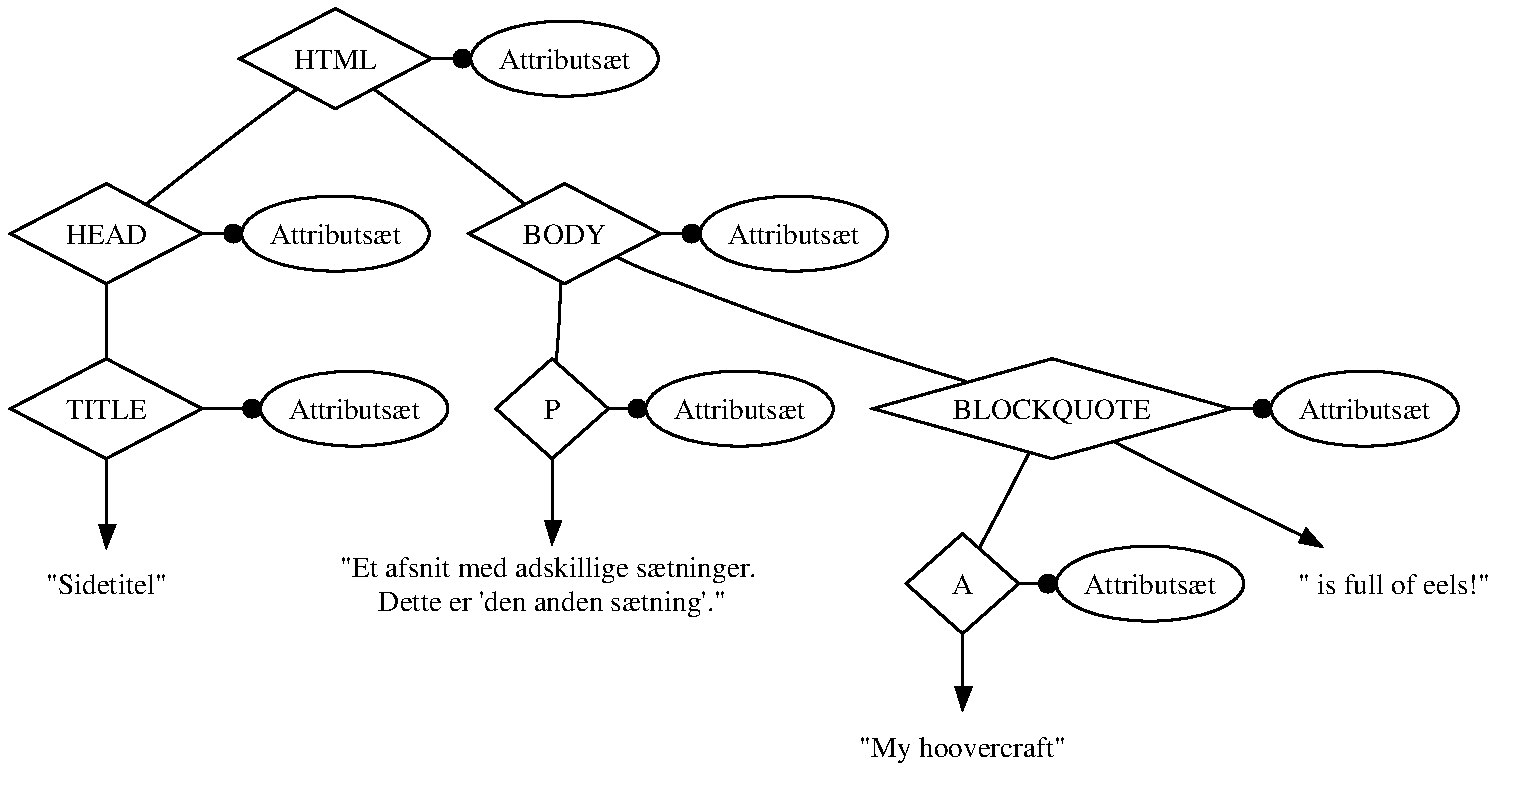
\includegraphics[width=\textwidth]{parsetree.pdf}
      \caption{Parsetræ}
    \end{figure}

    \pause

    \column{.5\textwidth}
    \begin{figure}
      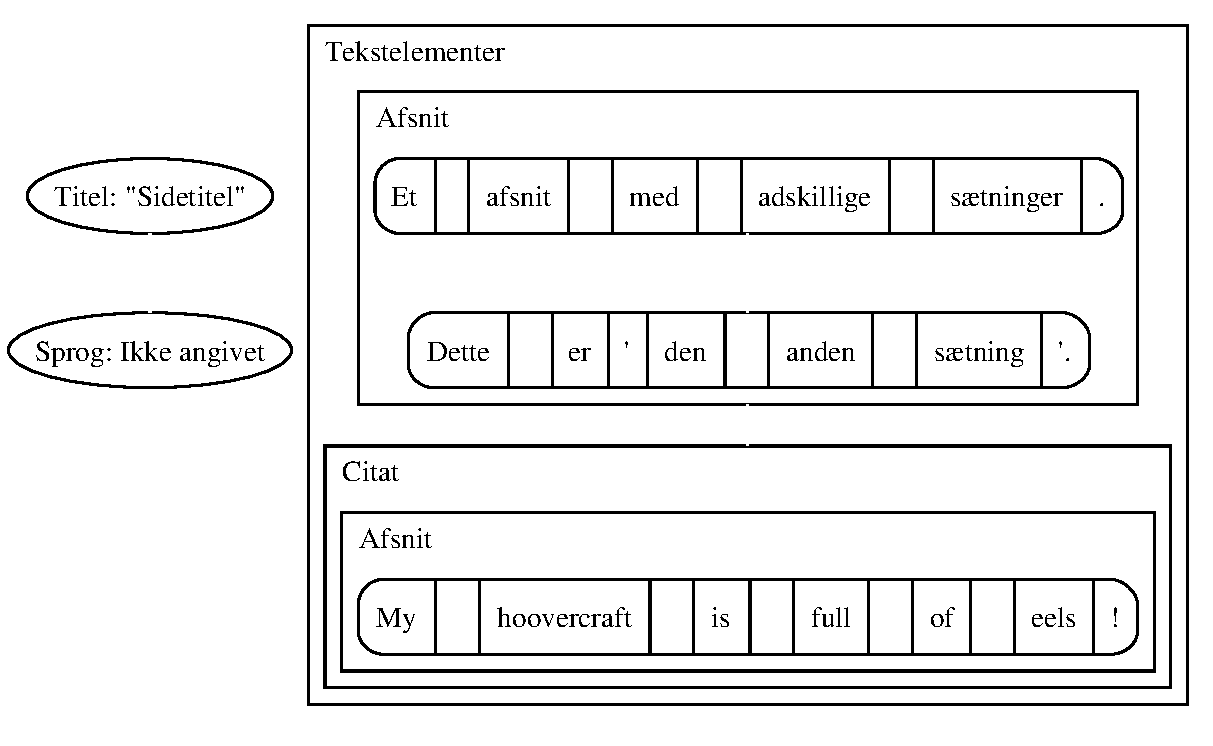
\includegraphics[width=\textwidth]{documentill.pdf}
      \caption{Dokument--struktur}
    \end{figure}
  \end{columns}
\end{frame}

\subsection{Tekstanalyse}
\begin{frame}
  \frametitle{Tekstanalyse}
  \framesubtitle{Analysemetoder}

  \begin{columns}[t]
    \column{.9\textwidth}

    \begin{block}{Beregning af Læsbarhedsindeks}
      \begin{displaymath}
        \frac{\text{antal ord}}{\text{antal sætninger}} +
        100\frac{\text{antal lange ord}}{\text{antal ord}}
      \end{displaymath}
    \end{block}


    \begin{block}{Beregning af Flesch Reading Ease}
      \begin{displaymath}
        206.835 - 1.015 \left ( \frac{\text{antal ord}}{\text{antal
              sætninger}} \right ) - 84.6 \left (
          \frac{\text{antal stavelser}}{\text{antal ord}} \right )
      \end{displaymath}
    \end{block}

    \begin{block}{Beregning af Flesch--Kincaid Grade Level}
      \begin{displaymath}
        0.39 \left ( \frac{\text{antal ord}}{\text{antal sætninger}} \right
        ) + 11.8 \left ( \frac{\text{antal stavelser}}{\text{antal ord}}
        \right ) - 15.59
      \end{displaymath}
    \end{block}

    \column{.1\textwidth}
    \end{columns}

\end{frame}

\begin{frame}
  \frametitle{Tekstanalyse}

  \begin{columns}[t]
    \column{.55\textwidth}
    \begin{figure}
      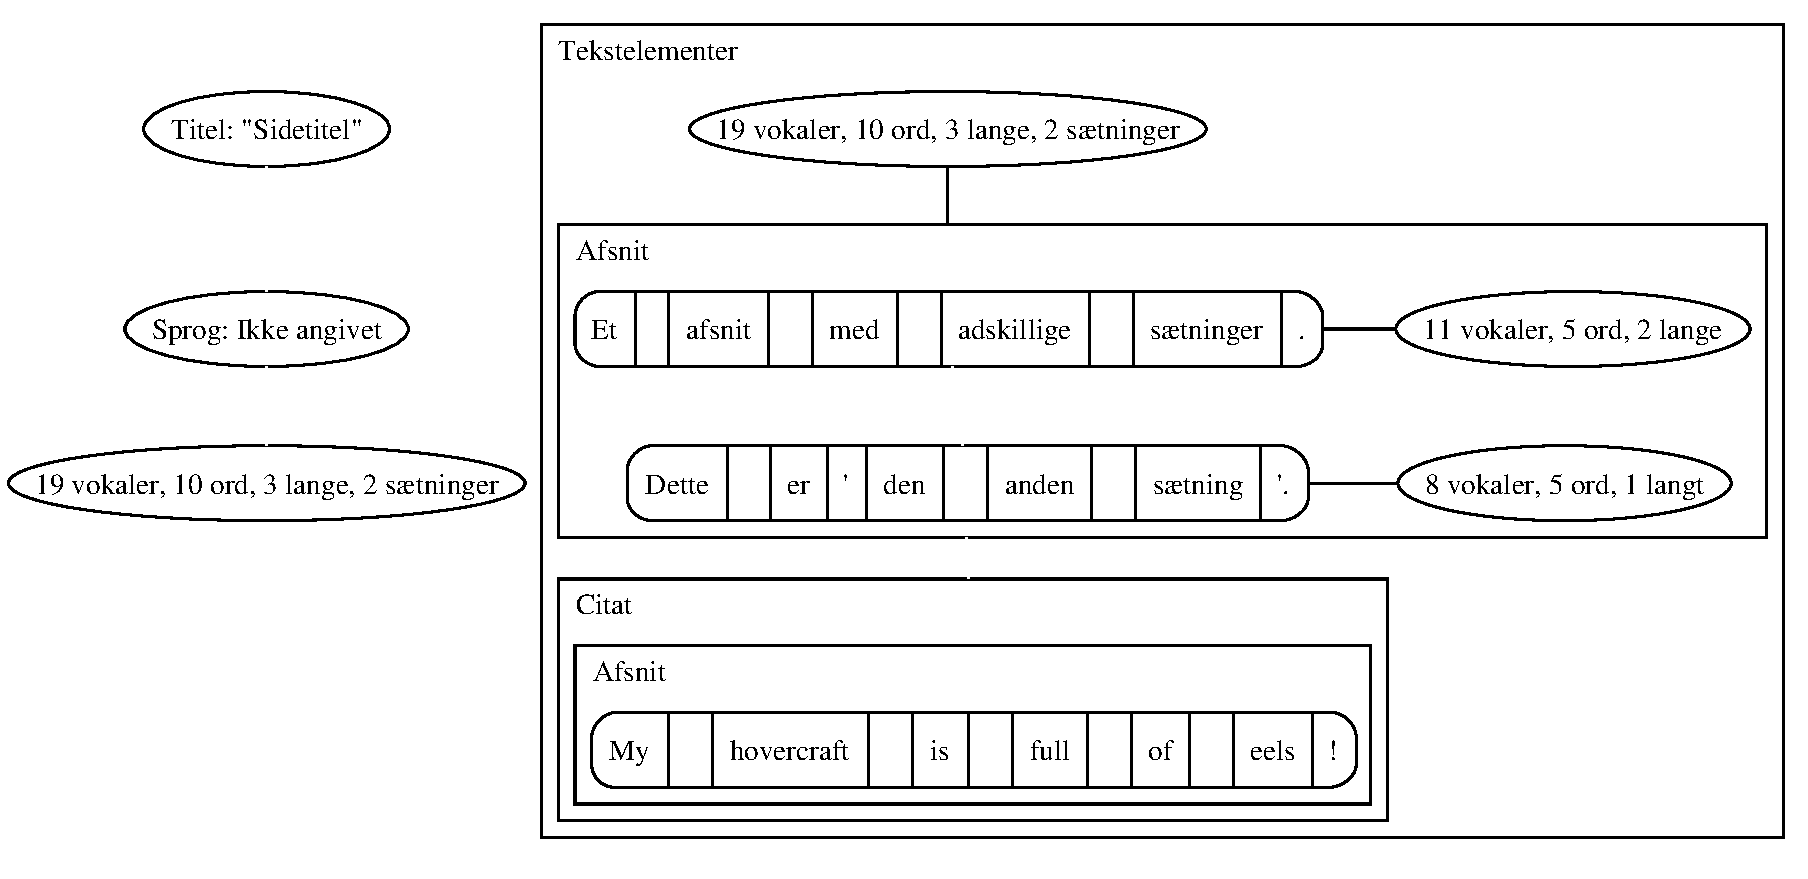
\includegraphics[width=\textwidth]{documentCount.pdf}
      \caption{Optælling}
    \end{figure}

    \column{.55\textwidth}
    \begin{figure}
      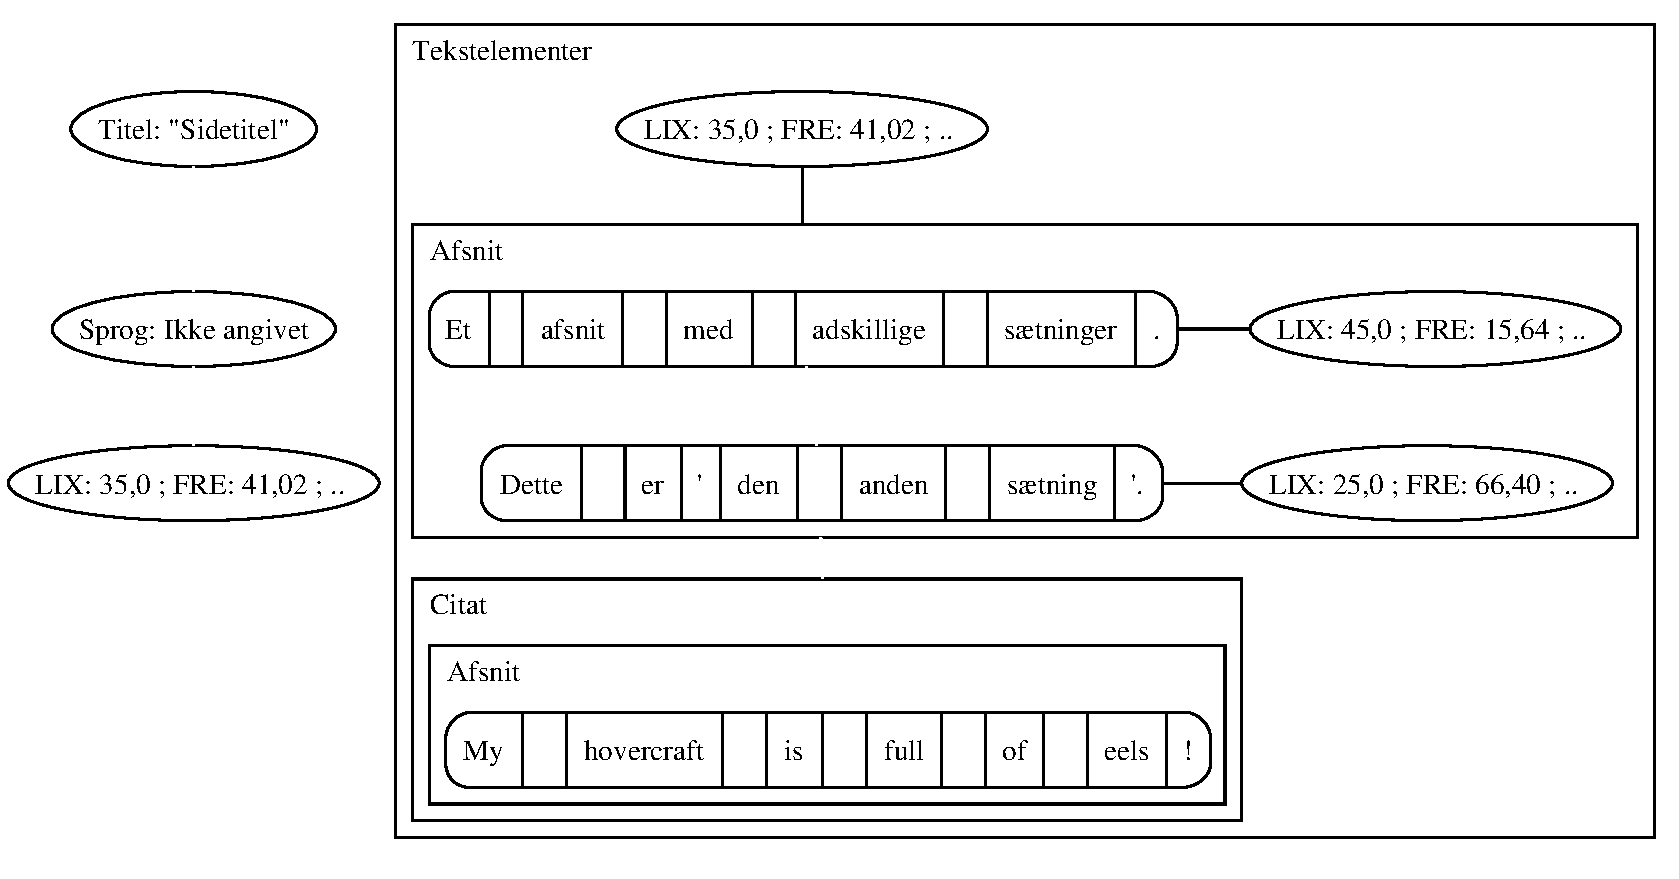
\includegraphics[width=\textwidth]{documentAnalyse.pdf}
      \caption{Analyseresultat}
    \end{figure}
  \end{columns}
\end{frame}

% \subsection{Crawling}
% \begin{frame}
%   \frametitle{Crawling}
%   \begin{itemize}
%   \item<1-> Dybde--først crawling kan give forkert resultat
%   \item<2-> Brug bredde--først og alt er vel
%   \end{itemize}
%   \begin{figure}
%     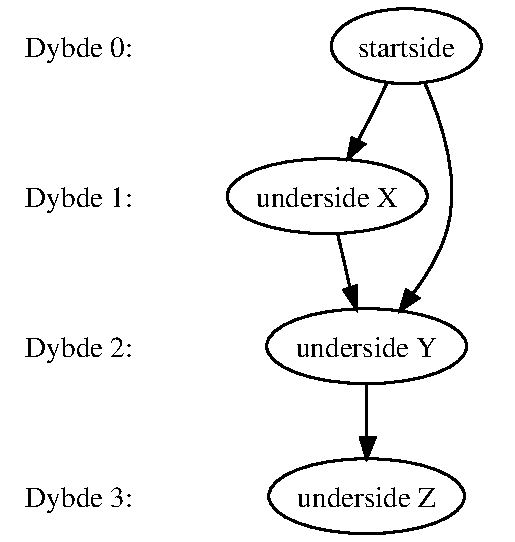
\includegraphics[width=0.55\textwidth]{depthtreeill.pdf}
%   \end{figure}
% \end{frame}


\section{Demonstration}
\subsection{Demonstration}
\begin{frame}
  \frametitle{Demonstration}
  \begin{figure}
    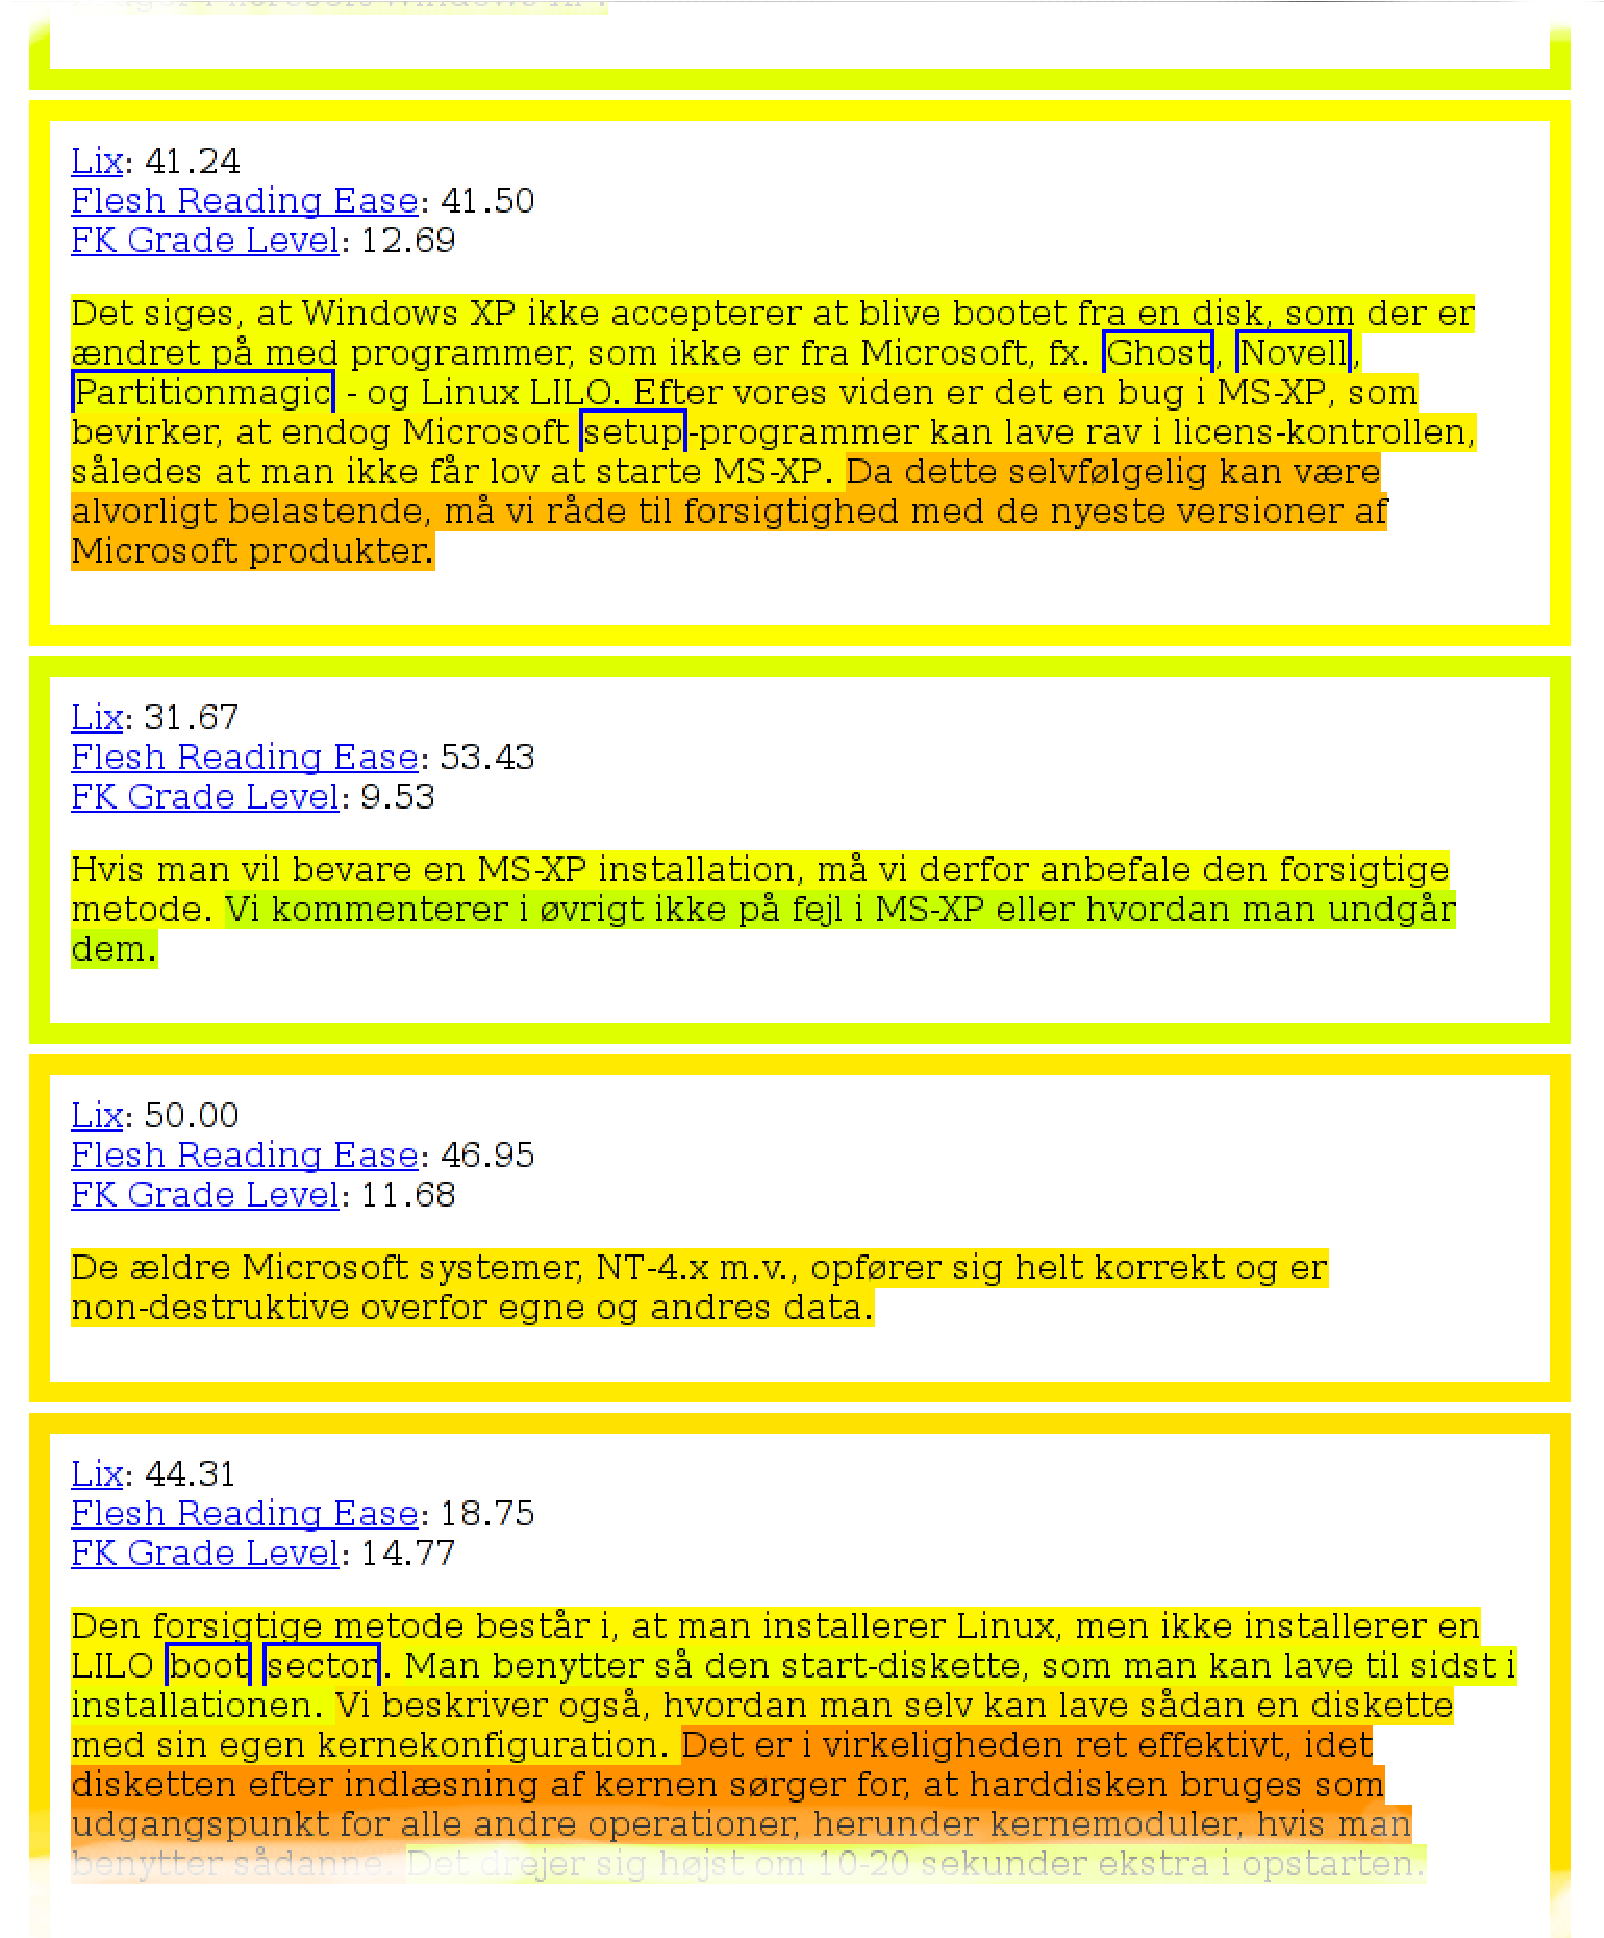
\includegraphics[width=0.55\textwidth]{webanalyzeroutput.pdf}
  \end{figure}
\end{frame}

\section{Afprøvning}
\subsection{Funktionstest}
\begin{frame}
  \frametitle{Funktionstest}

  \begin{block}{Skal afsløre\dots}
    \begin{itemize}
    \item \dots uopfyldte krav.
    \item \dots funktionalitet der ikke virker korrekt.
    \end{itemize}
  \end{block}

  Test kan ikke automatiseres, pga. uddatas format.

\end{frame}

\begin{frame}
  \frametitle{Funktionstest}
  \textbf{Fundne fejl}
    \begin{itemize}
    \item Det \textit{uundværlige} krav om håndtering af robots.txt
      (1.1), er kun delvist implementeret. Det er ikke muligt at slå
      robots.txt--behandlingen fra.

    \item \textbf{De resterende \textit{uundværlige} og \textit{vigtige}
      krav er implementeret korrekt.}

    \item Det \textit{mindre vigtige} krav (3) vedr. analysebaseret på
      HTML--tags er delvist implementeret.

    \item Det \textit{mindre vigtige} krav (4) om konfiguration af
      analyse er delvist implementeret. Filtrering på basis af
      \texttt{class}--attributer virker ikke.
    \end{itemize}
\end{frame}


\subsection{Brugertest}
\begin{frame}
  \frametitle{Brugertest}

  \begin{block}{Krav til forsøgsperson}
    \begin{itemize}
    \item Skal kende til elementær HTML.
    \item Skal kende til GNU/Linux, vores målplatformen.
    \item Skal have erfaring med kommandolinje programmer.
    \end{itemize}
  \end{block}
\pause

\textbf{Udførelse af test}
  \begin{itemize}
  \item Udført som tænk--højt forsøg.
  \item Vi valgte en person fra DIKU, da de fleste på DIKU har de 3
    ovenfor nævnte egenskaber.
  \item Vi stillede ham 3 opgaver og gav ham brugermanualen.
  \end{itemize}
\end{frame}

\begin{frame}
  \frametitle{Brugertest}
  \textbf{Resultater}
  \begin{itemize}
  \item Det er svært at se om programmet arbejder, om det er færdigt
    eller er gået i stå.
  \item Der mangler beskrivende tekst på indeks--siden, det er svært
    at se hvad farverne angiver og hvordan siderne er sorteret.
  \item Manualen var tvetydig omkring hvordan den maksimale dybde skal
    angives.
  \end{itemize}

\end{frame}

\section{Konklusion}
\subsection{Konklusion}
\begin{frame}
  \frametitle{Konklusion}

  \textbf{Status}

  \begin{itemize}
  \item<1-> Alle vigtige krav opfyldt
  \item<2-> Kun få krav ikke implementeret pga. tidsnød
  \item<3-> Kan udvides med flere analysemetoder og understøttelse af
    andre tekstformater.
  \item<4-> Programmet er ``brugbart''
  \end{itemize}
\pause
\pause
\pause
\pause
  \textbf{Problemer}

  \begin{itemize}
  \item<5-> Dårlig håndtering af tekstindkodning (indbefattet i krav)
  \item<6-> Sætningsopdeler ikke helt perfekt
    \begin{itemize}
    \item<6-> Kan let narres af forkortelser fulgt af navne
    \item<6-> Ingen egentlig dybdegående grammatisk forståelse
    \item<6-> Håndtering af ikke--angliske/nordiske sprog er mangelfuld
    \end{itemize}
  \item<7-> Respekt for \texttt{robots.txt} kan ikke slås fra
  \item<7-> Indeks--siden mangler forklaring af farver
%  \item<6-> Enkelttrådet program
  \end{itemize}
\end{frame}

\subsection{Perspektiver}
\begin{frame}
  \frametitle{Perspektiver}

  \textbf{Mulige udvidelser}

  \begin{itemize}
  \item<1-> Reel grammatisk forståelse baseret på det angivne sprog
  \item<2-> Flere analysemetoder, brugt/kombineret på mere intelligent måde
  \item<3-> Anden brugergrænseflade --- webapplikation eller grafisk applikation
  \item<4-> Læsbarhedsstatistik for websider --- gennemsnit, median, afvigelse, osv.
  \item<5-> Flertrådet program
  \end{itemize}
\end{frame}

\end{document}
